%%%%%%%%%%%%%%%%%%%%%%%%%%%%%%%%%%%%%%%%%%%%%%%%%%%%%%%%%%%%%%%%%%%%%%%%%%%%%%%%%%%
%%%%%%%%%%%%%%%%%%%%%%%%%%%%%%%%%%%%%%%%%%%%%%%%%%%%%%%%%%%%%%%%%%%%%%%%%%%%%%%%%%%
%                               START KAPITEL 1 
%%%%%%%%%%%%%%%%%%%%%%%%%%%%%%%%%%%%%%%%%%%%%%%%%%%%%%%%%%%%%%%%%%%%%%%%%%%%%%%%%%%
%%%%%%%%%%%%%%%%%%%%%%%%%%%%%%%%%%%%%%%%%%%%%%%%%%%%%%%%%%%%%%%%%%%%%%%%%%%%%%%%%%%

\section[Einführung]{Einführung in Schaltvorgänge}
\label{sec:einfuehrung}
\newvideofile{Einfuehrung}{Einführung in Schaltvorgänge}
\begin{frame}\ftx{\secname}
\s{%
	% Einführung 
	Schaltvorgänge sind Ausgleichsvorgänge, welche unmittelbar nach dem Schalten in elektrischen Netzwerken auftreten.
	Wie der Begriff \glqq elektrische Schaltung\grqq\ im Deutschen vermuten lässt, spielt das Schalten eine große Rolle in der Elektrotechnik. 
	Selbst elektrische Netzwerke, in denen nicht geschalten wird, werden gemeinhin als Schaltungen bezeichnet.

	% Beispiele
	Schalter finden vielfältig Anwendung unter anderem in der Leistungselektronik, der Informations-, der Kommunikations- 
	und der Regelungstechnik. Dabei kommt es nach jedem effektiven Schalten zu Ausgleichsvorgängen, 
	die mitunter erwünschte oder unerwünschte Effekte hervorrufen können.

	% Themen Eingrenzung
	In diesem Modul liegt der Fokus auf der Untersuchung dieser Ausgleichsvorgänge.
}
\begin{Lernziele}{\v{Video - }Einführung}
	Studierende lernen: 
	\begin{itemize}
		\item Schaltvorgänge als nicht-stationäre Zustände nach Schaltaktionen kennen % Wissen
		\item Schaltvorgänge im Kontext anderer Ausgleichsvorgänge zu verstehen % Verstehen
		\item Herausforderungen und Möglichkeiten bei Schaltvorgängen kennen % Wissen, Anwenden (Beispiele Praxis, LE, Filter, Verzögerungen, ...)
		\item das Schaltverhalten von idealen und realen Schaltern zu unterscheiden % Verstehen
	\end{itemize}
\end{Lernziele}
\speech{EinfuehrungLernziele}{1}{%
Sehr geehrte Studierende,
herzlich willkommen zum Video Einführung in Schaltvorgänge.
In diesem Video werden die Inhalte aus Kapitel 1 des Moduls Schaltvorgänge vorgestellt.
Hier sehen Sie die Lernziele des Kapitels und dieses Videos.

Anhand von Ausgleichsvorgängen im Allgemeinen mit einfachen Beispielen aus der Physik
werden wir den Begriff Schaltvorgang näher erläutern und Analogien heraus arbeiten.
Sie werden Ursachen, den typischen Ablauf und eine grobe Definition von Schaltvorgängen kennen lernen
und diese im größeren Zusammenhang mit anderen Ausgleichsvorgängen verstehen lernen. Anhand von Beispielen,
wo diese Auftreten und welche Auswirkungen möglich sind,
werden sie mögliche Herausforderungen sowie Möglichkeiten, die sich aus Schaltvorgängen ergeben kennen lernen.
Zudem lernen Sie Unterschiede im Verhalten von idealen und realen Schaltern kennen.
}% Speech Ende
\end{frame}

%%%%%%%%%%%%%%%%%%%%%%%%%%%%%%%%%%%%%%%%%%%%%%%%%%%%%%%%%%%%%%%%%%%%%%%%%%%%%%%%%%%%%%%%%%%%%%%%%%

\subsection{Ausgleichsvorgänge}
\label{sec:einfuehrung:ausgleichsvorgaenge}
\begin{frame}\ftx{\subsecname}
\s{%
	% Vorstellung: Ausgleichsvorgänge
	Ausgleichsvorgänge sind allgemein Vorgänge, in denen ein System nach einer Störung einem Gleichgewichtszustand zustrebt.
	
	% Analogien
	Ein Blick in die Physik zeigt, dass Ausgleichsvorgänge auf mannigfaltige Art und Weise in vielen Bereichen vorkommen. 
	Nach dem zweiten Hauptsatz der Thermodynamik strebt ein System stets einem Gleichgewichtszustand zu.
	Demnach kann jeder Vorgang bei entsprechenden Systemgrenzen als Ausgleichsvorgang betrachtet werden.
	Ein Stückweit lassen sich Schaltvorgänge mittels Analogien zu anderen Ausgleichsvorgängen beschreiben.  
	% Alle Vorgänge? 2. Satz Thermodynamik -> Makroskopisch? ... Mh...
	
	% Beispiele
	Beispiele für Ausgleichsvorgänge sind das Erhitzen einer Flüssigkeit, das Ausschwingen eines Pendels oder der Regelvorgang eines Regelkreises.

	\begin{figure}[H]\centering
		% Bild: Bartolomeo Pinelli, Ausschnitt aus \textit{A Peasant Family Cooking over a Campfire}, CC0 1.0. \url{https://commons.wikimedia.org/w/index.php?curid=81414513}
		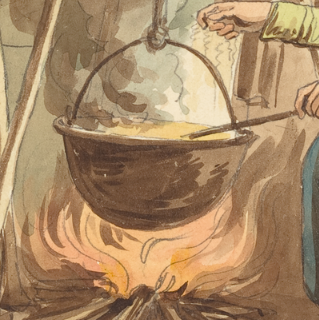
\includegraphics[width=0.3\textwidth]{Bilder/Ausschnitt_A_Peasant_Family_Cooking_over_a_Campfire_by_Bartolomeo_Pinelli_CC0_1.0.png} % 320x319px
		\caption{Erhitzen einer Flüssigkeit\protect\footnotemark}\label{fig:einfuehrung:ausgleichsvorgang:temperaturausgleich}
	\end{figure}
	\footnotetext{Bartolomeo Pinelli, Ausschnitt aus \textit{A Peasant Family Cooking over a Campfire}, Lizenz CC0 1.0\newline\qquad\url{https://commons.wikimedia.org/w/index.php?curid=81414513}}
		
	%Beispiel aperiodisch (DGL 1. Ordnung):\\
	%	Temperaturausgleich. Warum? Energieniveaus anschaulich und Irreversibilität (Entropiesteigerung) (klassisch)

	%Beispiel periodisch (DGL 2. Ordnung):\\
	%	Federpendel. Passt zu \glqq Einschwingvorgängen\grqq. (klassisch)

	%Beispiel periodisch (DGL 2. Ordnung):\\ 
	%	Vergleich Regelung (Motorik). Passt, weil rechnerisch gleich und abgedeckt in Definition ($\rightarrow$ stationärer Zustand)
	%	(Praktisch wegen Überschwingen)
}%
\b{%
	\begin{minipage}{\textwidth}% Obere Hälfte
		\begin{minipage}{0.48\textwidth}\centering
			\resizebox{0.9\textwidth}{!}{\includegraphics{Tikz/pdf/circ_switchable_rc_charge_dc.pdf}}
		\end{minipage}%
		\begin{minipage}{0.48\textwidth}\centering
			\includegraphics{Tikz/pdf/plot_rc_charge_uc_transition.pdf}
		\end{minipage}
	\end{minipage}
	\vspace{0.5cm}
	\pause

	\begin{minipage}{\textwidth}% Untere Hälfte
		\begin{minipage}[t]{0.48\textwidth}\centering
			\underline{Analogie: Wasser erhitzen}\footnotemark
			\vspace{2mm}

			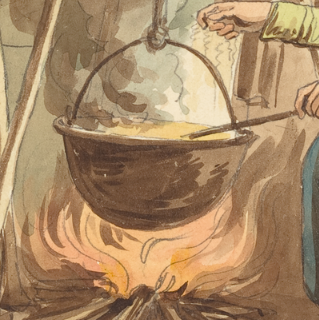
\includegraphics[width=0.4\textwidth]{Bilder/Ausschnitt_A_Peasant_Family_Cooking_over_a_Campfire_by_Bartolomeo_Pinelli_CC0_1.0.png}%
			\pause
		\end{minipage}%
		\begin{minipage}[t]{0.48\textwidth}%\centering
			\underline{Ursachen für Ausgleichsvorgänge:}
			\vspace{2mm}
			\begin{itemize}
				\item Schalthandlungen
				\item DC: Änderung d. Spannung/Strom
				\item AC: Änderung d. Frequenz/Amplitude/Phase
			\end{itemize}
		\end{minipage}
	\end{minipage}
	\footnotetext{Bild: Bartolomeo Pinelli, Ausschnitt aus \textit{A Peasant Family Cooking over a Campfire}, Lizenz CC0 1.0\newline\qquad\url{https://commons.wikimedia.org/w/index.php?curid=81414513}}
}%
\speech{EinfuehrungAusgleichsvorgaenge}{1}{%
Was sind nun Schaltvorgänge? Um diese Frage zu beantworten, fangen wir mit einem kleinem Beispiel an.
In der Schaltung links sehen wir eine R C Reihenschaltung.
Diese kann über einen Schalter entweder kurzgeschlossen werden oder an eine ideale Gleichspannungsquelle U q geschlossen werden.

Was passiert nun, wenn die Schalterstellung wechselt und die Spannung U q an die R C Reihenschaltung angeschlossen wird?

Ist die Kapazität zum Schaltzeitpunkt entladen (das heißt die Spannung u C an der Kapazität ist gleich null), so stellt sich der rechts zu sehende Zeitverlauf ein.
Wie zu sehen ist, steigt die Spannung u c an der Kapazität zunächst schnell und dann immer langsamer an und konvergiert am Ende gegen eine konstante Spannung.
Am Ende dieses Ladevorganges hat sich ein stationärer Zustand eingestellt.
Vor dem Schalten hatten wir ebenfalls einen stationären Zustand als die Kapazität vollständig entladen war.
Das was sich zwischen diesen beiden stationären Zuständen abspielt wird als Ausgleichsvorgang bezeichnet.
Von der angeschlossenen Spannungsquelle fließt solange Energie in die Kapazität, bis sich die Spannungen sich angeglichen haben.
Am Ende fließt kein Strom mehr und die Kapazität hat die Spannung U_q erreicht.
}% Speech Ende
\speech{EinfuehrungAusgleichsvorgaenge}{2}{%
Im Prinzip basieren alle makroskopischen Prozesse auf Ausgleichsvorgängen, je nachdem wie weit die Systemgrenzen gewählt werden.
Betrachten wir dieses Bild von einem Topf, der über einem Lagerfeuer erhitzt wird.
Nehmen wir an, der Topf ist mit Wasser gefüllt, das zunächst Umgebuntstemperatur hat.
Bei bei genügend Wärmezufuhr wird das Wasser anfangen zu kochen und schließlich unter Normaldruck eine konstante Temperatur von ungefähr hundert Grad Celsius erreichen.
Die zugeführte Energie entspricht dann exakt der abgeführten Energie (z.B. durch Verdunstung).
}%
\speech{EinfuehrungAusgleichsvorgaenge}{3}{%
Ursache für den Temperaturausgleich ist das Feuer machen unter dem Topf.
Analog dazu resultierte der Spannungsausgleich an der Kapazität durch den Anschluss der Gleichspannungsquelle.
Ursächlich für Ausgleichsvorgänge in Schaltungen sind plötzliche Änderungen in der Schaltung.
Zum Beispiel durch Schalthandlungen, bei DC-Netzwerken durch Änderung von Spannung oder Strom oder bei AC-Netzwerken durch Änderung von Amplitude, Frequenz oder Phase.
}% Speech Ende
\end{frame}

\b{% Beamer only, extra frame
\begin{frame}\ftx{\subsecname\,- Beispiele}
	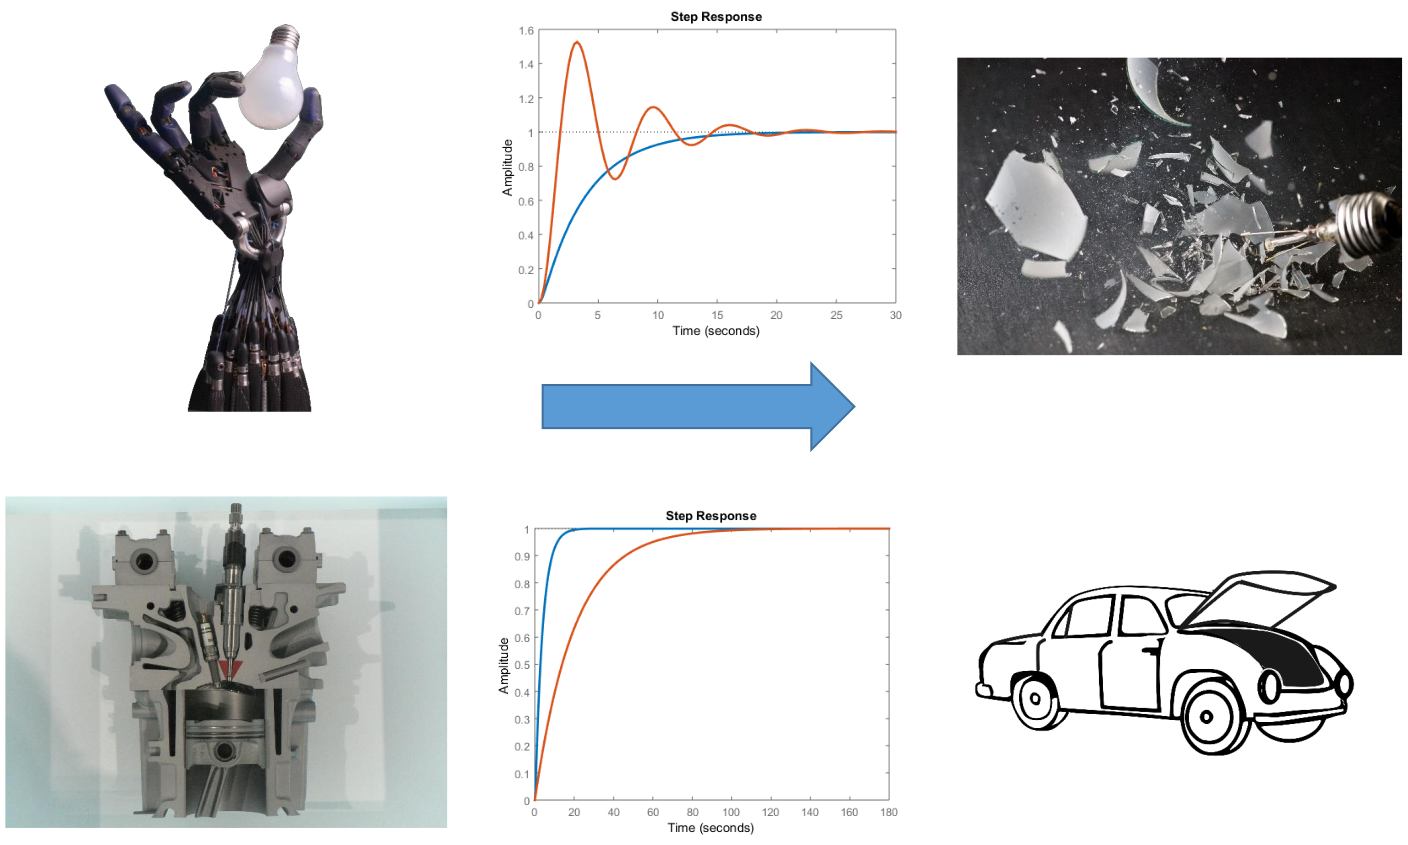
\includegraphics[width=\textwidth]{Bilder/Ausgleichsvorgaenge_Beispiele_ET3_S_Exknowski_FH_SWF.png}% Provisorisch mit Genehmigung von Prof. Exknowski
\speech{EinfuehrungAusgleichsvorgaengeBeispiele}{1}{%
Hier sind weitere Beispiele für ähnliches Systemverhalten. Auch Einschwingvorgänge bei Regelungsprozessen können als Ausgleichsvorgänge betrachtet werden. 

Im obigen Beispiel sehen wir einen Beispiel aus der Robotik.
Links zu sehen ist eine Roboterhand, die eine Glühbirne hält. 
Zum Halten, muss der Fingerdruck auf einen festen Wert regeln. 
Kommt es zu einem Überschwingen wie bei der orangenen Sprungantwort im mittleren Diagramm, kann dies den Bruch der Birne bedeuten
wie rechts im Bild angedeutet ist. Für eine feine Motorik muss das System schnell, aber auch präzise reagieren wie bei der blauen Sprungantwort ohne Überschwingen dargestellt ist. 

Im unteren Beispiel sehen wir ein Beispiel aus der Automobilindustrie. 
Links sehen wir den Querschnitt eines Verbrennungsmotors. Für ein angenehmes Fahrverhalten müssen Drehzahl- und Drehomentregelung stimmen.
Auch ohne Überschwingen kann eine zu abrupte Beschleunigung oder Abbremsung gerade beim Personentransport zu unerwünschten Folgen führen.

All diese Beispiele haben gemein, dass eine plötzliche Änderung, in diesem Fall durch den Sprung der Sollgröße im Regelkreis, einen Ausgleichsvorgang nach sich zieht.
Während der Ausgleichsvorgänge strebt die betrachtete Systemgröße einen stationären Zustand an. 
}% Ende Speech
\end{frame}
}
%%%%%%%%%%%%%%%%%%%%%%%%%%%%%%%%%%%%%%%%%%%%%%%%%%%%%%%%%%%%%%%%%%%%%%%%%%%%%%%%%%%%%%%%%%%%%%%%%%

\subsection{Schaltvorgänge}
\label{sec:einfuehrung:schaltvorgaenge}
\begin{frame}\ftx{\subsecname}
\s{
	% Def: Schaltvorgang, Prämisse (idealer Schalter)
	Als Schaltvorgänge werden Ausgleichsvorgänge unmittelbar \underline{nach} dem Schalten bezeichnet.
	Diese sind Hauptgegenstand des Moduls, wobei hierfür stehts von idealen Schaltern ausgegangen wird.

	% Bild: Schaltvorgang DC, AC
	Abbildung \ref{fig:plot:transient_persistent} zeigt exemplarisch den Zeitverlauf einer 
	Systemgröße $s(t)$ (z.B. Strom oder Spannung) während eines Schaltvorgangs. 
	Zum Vergleich sind für das Zuschalten einer Anregung zwei Fälle dargestellt:
	einmal für eine Gleichgröße (DC) und einmal für eine Wechselgröße (AC).
}
% Bsp. Einschwingvorgang nach Schalten als Schaltvorgang. Vgl. DC und AC 
\b{\centering Beispiel Schaltvorgang bei Gleich- und Wechselspannung.
}%
\fu{\includegraphics{Tikz/pdf/plot_transient_persistent.pdf}}%
	{Vergleich: Ausgleichsvorgang AC, DC\label{fig:plot:transient_persistent}}
\s{
	% Bild-Erklärung: Vorgänge, Zustände
	% stationär -> Schalten (instantan) -> Schaltvorgang (transient) -> stationärer Zustand (persistent)
	Der dargestellte Schaltvorgang beginnt mit dem Schalten bei $t=0$ (gestrichelte Grenze, links) 
	und endet mit Erreichen eines stationären Zustands (persistent) (gestrichelte Grenze, mittig).
	Der stationäre Zustand von $s(t)$ entspricht
	bei Anregung mit Gleichgröße (DC) ebenfalls einer Gleichgröße (konstant) und
	bei Anregung mit Wechselgröße (AC) ebenfalls einer Wechselgröße (periodisch). 

	Der in Abb. \ref{fig:plot:transient_persistent} dargestellte Vorgang beim Übergang (transient) 
	von Schalten bis Erreichen eines stationären Zustands kann hier auch als 
	Ausgleichsvorgang (allgemein), Schaltvorgang (speziell) oder Einschwingvorgang (speziell) bezeichnet werden. 

	% Abgrenzung: Vorgänge beim Schalten (realer Schalter)
	Ausgleichsvorgänge \underline{während} dem Schalten, wie sie bei realen Schaltern auftreten,
	werden nicht als Schaltvorgänge bezeichnet und in diesem Modul nicht näher untersucht. 
	Eine kurze Erläuterung findet sich jedoch vollständigkeitshalber in Abschnitt \ref{sec:einfuehrung:schalteridealvsreal} 
	beim Vergleich idealer und realer Schalter.
}%
\speech{EinfuehrungSchaltvorgaenge}{1}{%
 Hier sehen wir zwei Beispiele von Schaltvorgängen. Diese sind nichts anderes als Ausgleichsvorgänge in elektrischen Schaltungen,
 ausgelöst durch plötzliche Änderungen wie Schaltaktionen.
 Im obigen Beispiel sehen wir einen Einschwingvorgang bei Anregung mit einer Gleichspannung.
 Der Verlauf ähnelt dem Ladevorgang der Kapazität über den Widerstand. 
 Im unteren Beispiel sehen wir einen Einschwingvorgang bei Anregung mit einer Wechselspannung.
 In diesem Fall schwingt sich die Systemgröße s auf eine konstante Sinusform ein. 
 Mit den gepunkteten Verläufen wird angedeutet, wie sich der Zeitverlauf von s während des Schaltvorganges aus der
 Überlagerung einer Sinusschwingung wie im eingeschwungenen Zustand und einer Exponentialkurve wie im DC Fall ergibt. 
 Der Schaltvorgang bezeichnet den Zustand des Überganges bei dem ein stationärer Zustand angestrebt wird aber. 
 Stationär heißt im D C Fall ein konstanter Wert oder im A C Fall eine konstante Amplitude, Frequenz und Phase.
 Ausgleichsvorgänge werden insbesondere im Hochspannungsbereich oft Transienten genannt,
 abgeleitet vom lateinischen Wort *transire*, was zu Deutsch so viel wie *übergehen* bedeutet.
 Das Adjektiv *transient* bedeutet so viel wie übergangsweise. Das Gegenteil dazu ist *persistent*,
 vom lateinischen *persistere*, zu Deutsch *verharren*. 
 }% Speech Ende
\end{frame}

%%%%%%%%%%%%%%%%%%%%%%%%%%%%%%%%%%%%%%%%%%%%%%%%%%%%%%%%%%%%%%%%%%%%%%%%%%%%%%%%%%%%%%%%%%%%%%%%%%

\subsection{Beispiele für Schaltvorgänge}
\label{sec:einfuehrung:beispieleschaltvorgaenge}
\begin{frame}\ftx{\subsecname}
% Anwendungsbereiche von Schaltungstechnik: Leistungselektronik, Kommunikationstechnik(?), ...
\b{% Beamer only
\textbf{Beispiel aus der Leistungselektronik:} 

\begin{minipage}{0.38\textwidth}\centering
	\includegraphics[width=\textwidth]{Bilder/Tiefsetzsteller_Schaltung_GET2_J_Böcker_Uni_Paderborn_cut.png}
	Tiefsetzsteller mit Glättungskondensator\footnotemark
\end{minipage}%
\begin{minipage}{0.58\textwidth}\centering
	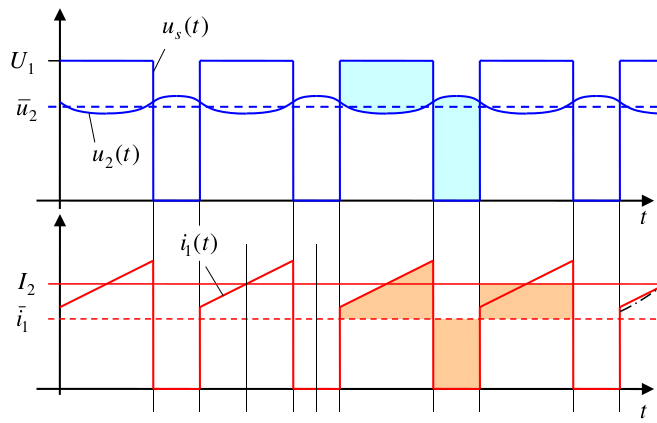
\includegraphics[width=0.9\textwidth]{Bilder/Tiefsetzsteller_Zeitverläufe_GET2_J_Böcker_Uni_Paderborn_cut_edit.png}
\end{minipage}
\footnotetext{Schaltbild und Zeitverlauf: Joachim Böcker, GET2, Universität Paderborn, modifiziert (gekürzt)}

Stromrichter (engl. \textit{power converter}) wandeln elektrische in elektrische Energie um 
Die Wandlung (z.B. Spannung, Strom, Frequenz) erfolgt durch getaktetes Schalten.\vspace{5pt}

\textbf{Andere Beispiele:}\\
Ein-/Ausschalten, AD-/DA-Converter, Fahrradlicht mit Kondensator, ...
}% end Beamer only
\s{% Skript only
	Prinzipiell kommt es bei jedem Schalten in elektrischen Netzwerken zu Schaltvorgängen. 
	
	Typische Beispiele sind Umrichter (engl. \textit{power converter}) in der Leistungselektronik,
	welche elektrische Energie in eine andere Form elektrischer Energie umwandeln. 
	Durch gezieltes Schalten von Halbleiterbauelementen (z.B. Transistoren, Thyristoren) 
	kann die Spannung, der Strom oder die Frequenz verändert werden. 
	In jedem Taktzyklus werden Kapazitäten und Indukivitäten abwechselnd geladen und entladen. 
	
	Abbildung \ref{fig:circ:pulldown} zeigt beispielhaft eine Tiefsetzsteller (Buck-Converter) mit Glättungskondensator.
	Dieser wandelt eine Gleichspannung $U_1$ in eine niedrigere Gleichspannung $U_2$ um. 
	Daneben sind in Abbildung \ref{fig:plot:pulldown} die zeitlichen Verläufe von Spannungen und Strömen
	jeweils am Eingang und am Ausgang des Tiefsetzstellers dargestellt.

	\begin{figure}[H]\centering
		\begin{subfigure}{0.5\textwidth}\centering
			\includegraphics[width=\textwidth]{Bilder/Tiefsetzsteller_Schaltung_GET2_J_Böcker_Uni_Paderborn_cut.png}
			\caption{Schaltbild eines Tiefsetzstellers (Buck-Converter)}
			\label{fig:circ:pulldown}
		\end{subfigure}%
		\begin{subfigure}{0.5\textwidth}\centering
			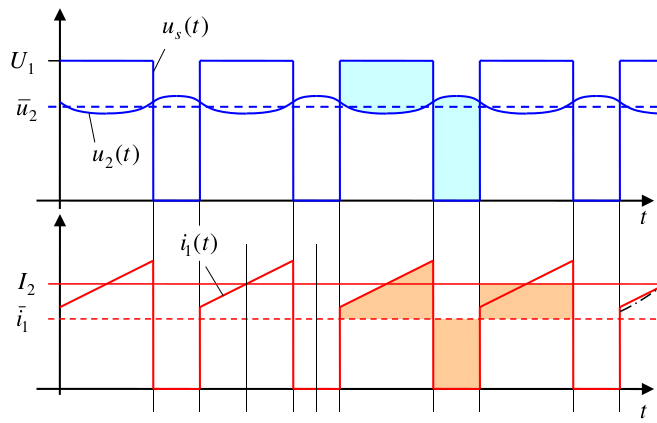
\includegraphics[width=0.9\textwidth]{Bilder/Tiefsetzsteller_Zeitverläufe_GET2_J_Böcker_Uni_Paderborn_cut_edit.png}
			\caption{Zeitverlauf von $u(t)$ und $i(t)$ am Tiefsetzsteller}
			\label{fig:plot:pulldown}
		\end{subfigure}
		\caption{Beispiel: Schaltvorgänge am Tiefsetzsteller\protect\footnotemark}
	\end{figure}
	\footnotetext{Quelle: Schaltbild und Zeitverlauf (modifiziert, gekürzt): Joachim Böcker, GET2, Universität Paderborn}

	Ohne nähere Rechnung ist erkennbar, dass die Ausgangsspannung auch im stationären Betrieb nicht konstant ist.
	Die Ausgangsspannung über dem Glättungskondensator schwankt, da sich die Kapazität in jeder Schaltperiode 
	etwas entlädt und wieder auflädt. 
	
	Mithilfe der Methoden aus diesem Modul lassen sich solche Schaltvorgänge berechnen und analysieren. 
	Zum besseren Verständnis werden in Kapitel \ref{sec:schaltvorgaengezeitbereich} jedoch einfachere Beispiele von
	Schaltvorgänge ohne periodisches Schalten betrachtet.

	Andere Beispiele für Schaltvorgänge sind das Ein- und Ausschalten von Geräten,
	Analog-Digital- und Digital-Analog-Wandlung, das Aufladen eines Kondensators durch ein Fahrradlicht.
}%
	%Bei elektrischen Schaltvorgängen: Schalter (Ein/Aus), Relais, Transistoren, ...
	%
	%Leistungselektronik überwiegend Schaltungselektronik im wortwörtlichen Sinne. 
	%%( DC <---DC/AC ---> AC)
	%%( î  .           .  î )
	%%( |    .       .    | )
	%%( |      .   .      | )
	%%(DC/DC     X     AC/AC)
	%%( |    .       .    | )
	%%( v  .           .  v )
	%%( DC <---DC/AC ---> AC)
	%
	%DC/AC: Wechselrichter (U,f,phi)\\
	%AC/AC: Frequenzumrichter (f) / Phasenregler (phi) / AC-Spannungsregler (U,(f),(phi))\\
	%DC/DC: Hochsetz-/Tiefsetz-/Hochtiefsetz-steller / DC-Spannungsregler (U)\\
	%AC/DC: Gleichrichter (U)\\
\speech{EinfuehrungSchaltvorgaengeBeispiele}{1}{%
Ein Bereich in dem es regelmäßig zu Schaltvorgängen kommt ist die Leistungselektronik.
In sogenannten Stromrichtern wird durch getaktetes Schalten elektrische Energie in eine andere Form elektrischer Energie gewandelt.
Im hier gezeigten Tiefsetzsteller wird beispielsweise die Gleichspannung U eins am Eingang in eine niedrigere Gleichspannung U zwei am Ausgang gewandelt. 
Das Spannungsverhältnis wird dabei durch den Tastgrad bestimmt, das heißt durch das Verhältnis von der Zeit bei geschlossenem Schalter 
während einer Periodendauer zur gesamten Periodendauer. 
In der oberen Schalterstellung lädt die Induktivität, wobei der Strom i L näherungsweise linear ansteigt und 
in der unteren Schalterstellung entlädt die Induktivität nährungsweise linear. 
Andere Beispiele in denen Schaltvorgänge auftreten sind zum Beispiel das Ein- und Ausschalten von elektrischen Geräten, 
die Änderung von Eingangssignalen bei A D und bei D A Convertern und Fahrradlampen mit Kondensator, wenn die Dynamospannung weg bricht. 
}% Speech Ende}
\end{frame}

%%%%%%%%%%%%%%%%%%%%%%%%%%%%%%%%%%%%%%%%%%%%%%%%%%%%%%%%%%%%%%%%%%%%%%%%%%%%%%%%%%%%%%%%%%%%%%%%%%

\subsection{Vergleich idealer und realer Schalter}
\label{sec:einfuehrung:schalteridealvsreal}
\begin{frame}\ftx{\subsecname}
\s{
	% Intro: Reales Schalten
	Zur Vereinfachung wird in diesem Modul stets von idealen Schaltern ausgegangen.
	Um die Grenzen dieser Annahme zu verstehen, wird im Folgenden der Unterschied zwischen idealen und realen Schaltern erläutert.
	Hierfür wird wie im Schaltbild in Abbildung \ref{fig:circ:switch} gezeigt ist, die Schalterspannung über einem Schalter betrachtet.
	Der Schalter ist hierfür an eine lineare Gleichspannungsquelle mit Spannung $U_q$ angeschlossen.
}
\begin{figure}[H]\centering
	\includegraphics{Tikz/pdf/circ_switch_ideal.pdf}
	\s{\caption{Schaltbild, Schalterspannung}}\b{\par Schalterspannung $\ecv{u(t)}$}
	\label{fig:circ:switch}
\end{figure}
\s{
	% Abbildung: Ideal vs. Real
	Abbildung \ref{fig:plot:schalter} zeigt die Schalterspannung im Durchlass- und im Sperrbetrieb und in den Übergangsphasen beim Öffnen oder Schließen des Schalters.
	Links ist der Spannungsverlauf für einen idealen Schalter dargestellt, rechts für einen realen Schalter.
}
\begin{figure}[H]\centering
	\begin{subfigure}{0.48\textwidth}\centering
		\includegraphics{Tikz/pdf/plot_switch_ideal.pdf}
		\s{\caption{Spannung bei idealem Schalter}}\b{\par Ideal: verlustlos, instantan}
		\label{fig:plot:schalter:ideal}
	\end{subfigure}\pause
	\begin{subfigure}{0.48\textwidth}\centering
		\includegraphics{Tikz/pdf/plot_switch_real.pdf}
		\s{\caption{Spannung bei realem Schalter}}\b{\par Real: Verluste, Latenzen}
		\label{fig:plot:schalter:real}
	\end{subfigure}
	\s{\caption{Vergleich: Schaltverläufe bei idealem und realem Schalter}}
	\label{fig:plot:schalter}
\end{figure}
%i(t),u(t)			ideal
%		î
%	U2_	|    ________         ______
%		|   |        |       |
%	U1_	|___|        |_______|
%		|___________________________> t
%
%i(t),u(t)			real
%		î
%	U2_	|..  _______   ....   ______    ___ = Spannung
%		|  ./       \.      ./
%	U1_	|__/ ....... \______/.......    ... = Strom
%		|___________________________> t
\speech{EinfuehrungSchalterIdealVsReal1}{1}{%
Für die Betrachtung von Schaltvorgängen werden im Rahmen des Moduls immer ideale Schalter angenommen. 
Ideale Schalter zeichnen sich dadurch aus, dass sie verlustlos und instantan schalten. 
Das bedeutet, dass Schaltaktionen sofort ohne Zeitverzögerung ausgeführt werden.
Im Durchlassbetrieb wird eine unendlich große Leitfähigkeit (wie ein Kurzschluss) angenommen und
im Sperrbetrieb wird ein unendlich großer elektrischer Widerstand (wie offene Klemmen) angenommen.
}% Speech Ende
\speech{EinfuehrungSchalterIdealVsReal1}{2}{%
In Realität kommt es bei realen Schaltern stets zu Verlusten und Latenzen. 
Im Durchlassbetrieb liegt immernoch eine kleine Spannung über dem nicht vernachlässigten Innenwiderstand an. 
Im Sperrbetrieb fließen immernoch kleine Ströme, wodurch ein Teil der Spannung über dem Innenwiderstand der Spannungsquelle abfällt. 
Aufgrund der Latenzen ändert sich die Schalterspannung nicht instantan in den Übergansphasen. 
Dadurch kommt es insbesondere während des Schaltens zu Verlusten, da bereits Ströme fließen während noch eine Spannung anliegt oder umgekehrt.
Die Latenzen und Verluste resultieren auf ohmschen, kapazitiven und induktiven parasitären Effekten wie gleich am Beispiel eines MOSFETs gezeigt wird.
}% Speech Ende
\end{frame}%

%-------------------------------------------------------------------------------------------------%

\begin{frame}\ftx{\subsecname}
\s{
	% Beschreibung: Ideal vs. Real
	Ein idealer Schalter wechselt beim Schalten instantan und verlustlos 
	von einem leitenden Zustand ($R=0$) zu einem sperrenden Zustand ($G=0$) oder umgekehrt
	wie in Abbildung \ref{fig:plot:schalter:ideal} dargestellt ist.
	Ein realer Schalter hingegen leitet oder sperrt nicht instantan
	wie in Abb. \ref{fig:plot:schalter:real} vereinfacht dargestellt ist. 
	Stattdessen treten Latenzen und Verluste auf.
	Im Durchlassbetrieb liegt immernoch eine kleine Spannung an (Durchlasswiderstand $R>0$)
	und im Sperrbetrieb fließt immernoch ein kleiner Strom (Sperrleitwert $G>0$).
	Dadurch kommt es zu Verlusten im Schalter, insbesondere während der Übergangsphasen, wenn sowohl Spannung als auch Strom anliegen.
	
	% Erklärung
	Die Latenzen und Verluste realer Schalter resultieren aus deren resistiven, induktiven und kapazitiven Eigenschaften.
	Aufgrund dieser Eigenschaften ist Schalten real betrachtet - schalterintern - immer mit Ausgleichsvorgängen verbunden.
	In der Praxis werden solche Effekte, wenn unerwünscht, als parasitär bezeichnet.
	
	% Beispiel: MOSFET
	Abbildung \ref{fig:circ:mosfet} zeigt exemplarisch einen MOSFET als Schalter zur Veranschaulichung. 
	Zum Vergleich ist der MOSFET einmal ideale (ohne) und einmal real (mit kapazitiven Effekten) dargestellt.
}
% Ref: http://fmh-studios.de/theorie/mosfet/schaltverhalten/
\begin{figure}[H]\centering
	\begin{subfigure}{0.48\textwidth}\centering
		\includegraphics{Tikz/pdf/circ_mosfet_ideal.pdf}
		\s{\caption{MOSFET, ohne Kapazitäten (ideal)}}\b{Ideal: keine parasitären Effekte}
		\label{fig:circ:mosfet:ideal}
	\end{subfigure}%
	\onslide<2->{%
	\begin{subfigure}{0.48\textwidth}\centering
		\includegraphics{Tikz/pdf/circ_mosfet_capacitive_effects.pdf}
		\s{\caption{MOSFET, inkl. Kapazitäten (real)}}\b{Real: mit parasitären Kapazitäten}
		\label{fig:circ:mosfet:kapazitiv}
	\end{subfigure}
	}% end onslide
	\s{\caption{Vergleich: Schaltung mit MOSFET, ohne (ideal) und mit kapazitiver Effekte (real)}}
	\label{fig:circ:mosfet}
\end{figure}
	%Alt. Bildbeschreibung:
	%Zwei Schaltbilder eines MOSFET, links ideal, rechts realer.
	%MOSFET Anschlüsse Gate G, Drain D und Source S jeweils wie folgt angeschlossen.
	%D über Widerstand R mit konstant 5 V versorgt.
	%S auf 0 V gelegt. 
	%Eingangsspannung U_1 zwischen G und S,
	%Ausgangsspannung U_2 zwischen D und S.
	%Realer MOSFET zusätzlich mit Kapazitäten zwischen allen drei Anschlüssen G, S und D.
\s{

	% Erklärung Latenzen, Abgrenzung
	Die kapazitiven Effekte zwischen den Anschlüssen des MOSFETs führen zu einer Verzögerung beim Schalten,
	da die jeweiligen Kapazitäten während des Schaltens erst geladen beziehungsweise entladen werden müssen.
	Das MOSFET-Beispiel dient lediglich zur Veranschaulichung der Unterschiede zwischen idealen und realen Schaltern.
	Ausgleichsvorgänge während Schaltaktionen werden in diesem Modul nicht weiter betrachtet.
	Mit Schaltvorgängen sind immer die Ausgleichsvorgänge \underline{nach} dem Schalten gemeint.
}%
\b{%
	\makebox[2cm][l]{\textbf{Hier:}} Ausgleichsvorgänge \makebox[1.5cm][c]{\underline{nach}} Schalten (Schaltvorgänge) im Fokus
	%\\\qquad$\rightarrow$ Annahme idealer Schalter %(verlustlos, instantan)
	\\[+4pt]%
	\makebox[2cm][l]{\textbf{Real:}} Ausgleichsvorgänge \makebox[1.5cm][c]{\underline{während}} Schalten
	%\\\qquad$\rightarrow$ Schaltverluste und Latenzen
	\\[+4pt]%
	\makebox[2cm][l]{\textbf{Eingrenz.:}} Annahme idealer Schalter 
}%
\speech{EinfuehrungSchalterIdealVsReal2}{1}{%
Links sehen wir das Schaltbild eines MOSFET Schalters mit Gain, Drain und Source Anschlüssen.
Ideal betrachtet treten keine paraisären Effekte auf.
}% Speech Ende
\speech{EinfuehrungSchalterIdealVsReal2}{2}{%
Real betrachtet treten kapazitive Effektische zwischen allen drei Anschlüssen auf.
Das führt dazu, dass die Gate-Source Spannung, um den Schalter zu Öffnen oder zu Schließen sich nicht instantan ändern kann.
Bevor der MOSFET seinen Zustand zwischen Sperren und Durchlass wechselt, müssen die Kapazitäten erst entladen oder geladen werden,
wodurch Latenzen beim Schalten entstehen.
Im Rahmen des Moduls fokussieren wir uns ausschließlich auf Schaltvorgänge, das heißt auf die Ausgleichsvorgänge *nach* dem Schalten.
Real betrachtet kommt es bereits während des Schaltens zu Ausgleichsvorgängen innerhalb der jeweiligen Schalter.
Zur Vereinfachung werden in diesem Modul stets ideale Schalter angenommen.
}% Speech Ende
\end{frame}